%%%%%%%%%%%%%%%%%%%%%%%%%%%%%%%%%%%%%%%%%%%%%%%%%
%%%%%%%%%%%%%%%%%%% EXAMPLE 3 %%%%%%%%%%%%%%%%%%%
%%%%%%%%%%%%%%%%%%%%%%%%%%%%%%%%%%%%%%%%%%%%%%%%%

% Minimal example of a PhD manuscript, in English
% Compile with: latexmk -lualatex -outdir=build main_phd.tex
% Compared with "main_hdr.tex", the "phd" option changes the diploma name on the cover,
% and expects a single jury list (with an explicit role per member) instead of reviewers/examiners

%%%%%%%%%%%%%%%%%%%%%%%%%%%%%%%%%%%%%%%%%%%%%%%%%
%%%%%%%%%%%%%%%%% CONFIGURATION %%%%%%%%%%%%%%%%%
%%%%%%%%%%%%%%%%%%%%%%%%%%%%%%%%%%%%%%%%%%%%%%%%%

% Choose template
\documentclass[phd, english]{template/hdr}

%%%%%%%%%%%%%%%%%%%%%%%%%%%%%%%%%%%%%%%%%%%%%%%%%
%%%%%%%%%%%%%%%%%% INFORMATION %%%%%%%%%%%%%%%%%%
%%%%%%%%%%%%%%%%%%%%%%%%%%%%%%%%%%%%%%%%%%%%%%%%%

% Author
\setAuthorFirstName{Fourth}
\setAuthorName{Student}

% Affiliations
\setUniversity{Placeholder University}
\setDoctoralSchool{Placeholder Doctoral School}
\setDoctoralSchoolSubtitle{Information Sciences \& Technologies}
\addLogo{manuscript/covers/logo_university.png}{https://example.org}
\addLogo{manuscript/covers/logo_doctoral_school.png}{https://example.org}
\addLogo{manuscript/covers/logo_laboratory.png}{https://example.org}

% Document
\setDocumentTitle{A Placeholder Title for a Placeholder Thesis}
\setDefenseDate{2026-09-30}

% Jury
% For a PhD, all members are in a single list, the last argument being their role
\addJuryMember{Firstname}{Reviewerone}{Senior Researcher, \acro{hdr}}{Placeholder Laboratory, Placeholder University}{Reviewer}
\addJuryMember{Firstname}{Reviewertwo}{Professor, \acro{hdr}}{Placeholder Institute}{Reviewer}
\addJuryMember{Firstname}{Examinerone}{Researcher, \acro{hdr}}{Placeholder Institute}{Examiner}
\addJuryMember{Firstname}{Lastname}{Associate Professor, \acro{hdr}}{Placeholder Laboratory}{Supervisor}
\addJuryMember{Second}{Coauthor}{Researcher}{Placeholder Laboratory}{Co-supervisor}

% Back cover elements
\setQRCodeLink{https://github.com/BastienPasdeloup/HDR-Template}
\setBackText{
    This text appears on the back cover, spread over two columns. Replace it with the abstract of your thesis. Lorem ipsum dolor sit amet, consectetur adipiscing elit, sed do eiusmod tempor incididunt ut labore et dolore magna aliqua. Ut enim ad minim veniam, quis nostrud exercitation ullamco laboris nisi ut aliquip ex ea commodo consequat. Duis aute irure dolor in reprehenderit in voluptate velit esse cillum dolore eu fugiat nulla pariatur. Excepteur sint occaecat cupidatat non proident, sunt in culpa qui officia deserunt mollit anim id est laborum. Sed ut perspiciatis unde omnis iste natus error sit voluptatem accusantium doloremque laudantium, totam rem aperiam, eaque ipsa quae ab illo inventore veritatis et quasi architecto beatae vitae dicta sunt explicabo.}

% Bibliography
% A PhD manuscript usually cites more external work than it lists own publications
% Here we keep a single category: in that case, the letter code and the category
% title are not used, and all entries appear in a single list
% Beware: every category cited in the text must be declared, otherwise compilation fails
\addBiblioCategory{journal}{J}{Journals}

%%%%%%%%%%%%%%%%%%%%%%%%%%%%%%%%%%%%%%%%%%%%%%%%%
%%%%%%%%%%%%%%%%%%%% CONTENT %%%%%%%%%%%%%%%%%%%%
%%%%%%%%%%%%%%%%%%%%%%%%%%%%%%%%%%%%%%%%%%%%%%%%%

% Go
\begin{document}

% Start with table of contents
\tableofcontents

% Chapters
\chapter[phd_introduction]{Introduction}
 [
  A PhD manuscript uses exactly the same commands as an HDR one: only the \texttt{phd} option of the document class differs. \\
  This chapter introduces the placeholder problem addressed in this thesis, and outlines the rest of the document.
 ]

\section[phd_context]{Context}

Lorem ipsum dolor sit amet, consectetur adipiscing elit, sed do eiusmod tempor incididunt ut labore et dolore magna aliqua~\cite{ipsum1998foundational}.
Ut enim ad minim veniam, quis nostrud exercitation ullamco laboris nisi ut aliquip ex ea commodo consequat~\cite{tempor2009textbook}.

The rest of this document uses \acro{ml} vocabulary, and in particular the \acrofull{cnn}.
Note that \acro{cnn_plural} is a separate entry of \verb|acronyms.tex|, whose only purpose is to provide a plural tooltip: its full name is \acroname{cnn_plural}, and it does not appear in the list of acronyms.
Recall that \acrofull{sota} results in this placeholder field are due to \cite{amet2017seminal}.

\section[phd_problem]{Problem Statement}

\begin{boxenv}[phd_problem_box]{Problem}[Placeholder problem]
    Given a set of placeholder observations $\{\bm{x}_i\}_{i = 1}^N$ and their placeholder targets $\{\bm{y}_i\}_{i = 1}^N$, find a placeholder model $f_\theta$ that generalizes to unseen placeholder observations.
\end{boxenv}

Duis aute irure dolor in reprehenderit in voluptate velit esse cillum dolore eu fugiat nulla pariatur.
\nameref{phd_problem_box} is addressed in \nameref{phd_contribution}, after the review of \nameref{phd_state_of_the_art}.

\section[phd_outline]{Outline}

\nameref{phd_state_of_the_art} reviews the placeholder literature.
\nameref{phd_contribution} presents our contribution, evaluated in \nameref{phd_contribution_results}.
\nameref{phd_conclusion} concludes, and \nameref{phd_proofs} gathers the proofs.

\chapter[phd_state_of_the_art]{State of the Art}
[
    This chapter reviews the placeholder literature, and positions the contribution of \nameref{phd_contribution} with respect to it.
]

    \section[phd_sota_early]{Early Approaches}

        Lorem ipsum dolor sit amet, consectetur adipiscing elit~\cite{ipsum1998foundational}.
        Sed do eiusmod tempor incididunt ut labore et dolore magna aliqua, as summarized in the textbook of \cite{tempor2009textbook}.

        \begin{boxenv}[phd_definition]{Definition}[Placeholder representation]
            A \emph{placeholder representation} of an observation $\bm{x}$ is any vector $\bm{z} = g(\bm{x})$ such that $\bm{z}$ carries no more information than $\bm{x}$.
        \end{boxenv}

    \section[phd_sota_modern]{Modern Approaches}

        Ut enim ad minim veniam, quis nostrud exercitation ullamco laboris nisi ut aliquip ex ea commodo consequat~\cite{amet2017seminal}.
        \acro{cnn_plural} are now trained on a single \acro{gpu}, which was not the case for the earlier approaches of \nameref{phd_sota_early}.
        \nameref{phd_sota_figure} summarizes the pipeline they all share.

        \begin{figure}[phd_sota_figure]{An overview of the placeholder pipeline shared by modern approaches. The same figure is reused in \nameref{phd_contribution}, which is perfectly fine as long as the labels differ.}
            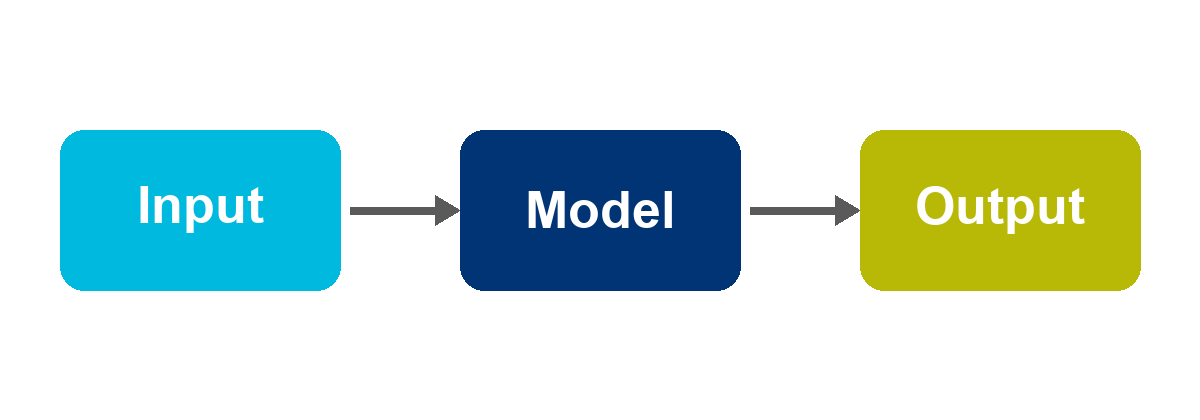
\includegraphics[width=0.9\linewidth]{manuscript/figures/example_diagram.png}
        \end{figure}

    \section[phd_sota_summary]{Summary}

        \nameref{phd_sota_table} compares the approaches discussed above.
        None of them addresses \nameref{phd_problem_box} directly, which motivates the contribution of \nameref{phd_contribution}.

        \begin{table}[phd_sota_table]{A comparison of placeholder approaches. Checkmarks are placeholders too.}
            \begin{tabular}{lccc}
                \hline
                \textbf{Approach} & \textbf{Placeholder} & \textbf{Scalable} & \textbf{Interpretable} \\
                \hline
                \cite{ipsum1998foundational} & \faCheck & \faTimes & \faCheck \\
                \cite{tempor2009textbook} & \faCheck & \faTimes & \faTimes \\
                \cite{amet2017seminal} & \faCheck & \faCheck & \faTimes \\
                \textbf{Ours} & \faCheck & \faCheck & \faCheck \\
                \hline
            \end{tabular}
        \end{table}

\chapter[phd_contribution]{A Placeholder Contribution}
 [
  This chapter presents the contribution of this thesis, and is the one that demonstrates most of the environments provided by the template. \\
  It answers \nameref{phd_problem_box}, stated in \nameref{phd_introduction}.
 ]

\section[phd_contribution_method]{Method}

We look for a placeholder model $f_\theta$ minimizing the objective of \nameref{phd_contribution_loss}, where $\lambda > 0$ controls the strength of the placeholder regularizer.

\begin{equation}[phd_contribution_loss]
    \mathcal{L}(\theta) = \underbrace{\frac{1}{N} \sum_{i = 1}^{N} \left\| f_\theta(\bm{x}_i) - \bm{y}_i \right\|_2^2}_{\text{placeholder fidelity}} + \lambda \underbrace{\left\| \theta \right\|_2^2}_{\text{placeholder regularizer}}
\end{equation}

\begin{boxenv}[phd_proposition]{Proposition}[Existence of a placeholder minimizer]
    For every $\lambda > 0$, the objective of \nameref{phd_contribution_loss} admits at least one minimizer $\theta^\star$.
\end{boxenv}

The proof of \nameref{phd_proposition} is deferred to \nameref{phd_proofs}, so as not to interrupt the exposition.
An unnumbered equation is obtained with the starred variant, which is convenient for intermediate steps:

\begin{equation*}
    \nabla_\theta \mathcal{L}(\theta) = \frac{2}{N} \sum_{i = 1}^{N} \left( f_\theta(\bm{x}_i) - \bm{y}_i \right) \nabla_\theta f_\theta(\bm{x}_i) + 2 \lambda \theta
\end{equation*}

\section[phd_contribution_results]{Results}

We evaluate the method of \nameref{phd_contribution_method} on placeholder datasets.
\nameref{phd_results_figure} reports the learning curves, and \nameref{phd_results_table} the final scores.

\begin{figure}[phd_results_figure]{Placeholder results. \nameref{phd_results_figure_curves} reports the metric along training, while \nameref{phd_results_figure_qualitative} shows a qualitative example.}
    \begin{subfigure}[phd_results_figure_curves]{0.52\linewidth}{Placeholder metric along training, for our model and the baseline of \cite{amet2017seminal}.}
        % Example of a vector figure, meant to be included with \input{} inside a figure environment
% Such fragments are typically produced by a script, so that data and rendering stay in sync
% The tikzpicture environment is patched by the template to never overflow \linewidth

\begin{tikzpicture}

    \begin{axis}
        [
            height      = 5cm,
            width       = \linewidth,
            xlabel      = {Number of training epochs},
            ylabel      = {Placeholder metric},
            xmin        = 0, xmax = 20,
            ymin        = 0, ymax = 1,
            grid        = major,
            grid style  = {separatorColor},
            legend pos  = south east,
            legend cell align = left,
        ]

        \addplot[titlesColor, line width=1.5pt, mark=*, mark size=1.5pt] coordinates
            {
                (0, 0.10) (2, 0.38) (4, 0.55) (6, 0.66) (8, 0.73)
                (10, 0.78) (12, 0.82) (14, 0.84) (16, 0.86) (18, 0.87) (20, 0.87)
            };
        \addlegendentry{Placeholder model}

        \addplot[linksColor, line width=1.5pt, dashed, mark=square*, mark size=1.5pt] coordinates
            {
                (0, 0.10) (2, 0.30) (4, 0.44) (6, 0.53) (8, 0.59)
                (10, 0.63) (12, 0.66) (14, 0.68) (16, 0.69) (18, 0.70) (20, 0.70)
            };
        \addlegendentry{Placeholder baseline}

    \end{axis}

\end{tikzpicture}

    \end{subfigure}
    \hfill
    \begin{subfigure}[phd_results_figure_qualitative]{0.44\linewidth}{A qualitative placeholder example.}
        
\includegraphics[width=\linewidth]{manuscript/figures/example_image.png}
    \end{subfigure}
\end{figure}

\begin{table}[phd_results_table]{Final placeholder scores, averaged over five placeholder runs. Best results in bold.}
    \begin{tabular}{lcc}
        \hline
        \textbf{Dataset} & \textbf{\cite{amet2017seminal}} & \textbf{Ours}        \\
        \hline
        Placeholder-A    & $0.70 \pm 0.02$                 & $\bm{0.87 \pm 0.01}$ \\
        Placeholder-B    & $0.61 \pm 0.03$                 & $\bm{0.79 \pm 0.02}$ \\
        Placeholder-C    & $0.55 \pm 0.04$                 & $\bm{0.68 \pm 0.03}$ \\
        \hline
    \end{tabular}
\end{table}

Excepteur sint occaecat cupidatat non proident, sunt in culpa qui officia deserunt mollit anim id est laborum.
These results were partly published in \cite{lastname2021journal} and \cite{lastname2024journal}.

\section[phd_contribution_discussion]{Discussion}

\begin{boxenv*}{\faExclamationTriangle~Limitations}
    An unnumbered box, obtained with \texttt{boxenv*}, is handy for remarks that do not need to be cross-referenced.
    The placeholder method has placeholder limitations, which are discussed in \nameref{phd_conclusion}.
\end{boxenv*}

\chapter[phd_conclusion]{Conclusion \& Perspectives}
[
    A short closing chapter, summarizing the contribution of \nameref{phd_contribution} and listing the directions it opens.
]

    \section[phd_conclusion_summary]{Summary}

        This thesis addressed \nameref{phd_problem_box}, introduced in \nameref{phd_introduction}.
        After the review of \nameref{phd_state_of_the_art}, \nameref{phd_contribution} proposed a placeholder method, whose objective is given in \nameref{phd_contribution_loss} and whose results are reported in \nameref{phd_results_table}.

    \section[phd_conclusion_perspectives]{Perspectives}

        \begin{itemize}
            \item Extending the placeholder method to placeholder data of higher dimension.
            \item Reducing the \acro{gpu} cost of placeholder training, so that the approach scales beyond placeholder datasets.
            \item Studying the interpretability of the placeholder representations of \nameref{phd_definition}.
        \end{itemize}

        Lorem ipsum dolor sit amet, consectetur adipiscing elit, sed do eiusmod tempor incididunt ut labore et dolore magna aliqua.


% Appendices
\appendices
% Appendix of the PhD example: chapters after \appendices are numbered as appendices
\chapter[phd_proofs]{Proofs}
 [
  Deferring proofs to an appendix keeps the main text readable. \\
  The \texttt{proof} environment takes the label of the statement it proves, and displays a clickable reference to it in its title.
 ]

\section[phd_proofs_proposition]{Existence of a Placeholder Minimizer}

\begin{proof}{phd_proposition}
    The objective of \nameref{phd_contribution_loss} is continuous in $\theta$, and coercive as soon as $\lambda > 0$, since $\left\| \theta \right\|_2^2 \to \infty$ when $\left\| \theta \right\|_2 \to \infty$.
    A continuous coercive function on $\mathbb{R}^d$ attains its infimum, hence the existence of a minimizer $\theta^\star$.
\end{proof}

\section[phd_proofs_misc]{A Proof Without a Statement}

The mandatory argument of \texttt{proof} can also be left empty, in which case the box is simply titled \inquotes{Proof}.

\begin{proof}{}
    Lorem ipsum dolor sit amet, consectetur adipiscing elit, sed do eiusmod tempor incididunt ut labore et dolore magna aliqua.
\end{proof}


% Bibliography and glossary at the end
\printbibliography
\printglossaries

% Done
\end{document}
